\documentclass{article}

% Essential packages
\usepackage{graphicx}   % For image handling
\usepackage{subcaption} % For multi images
\usepackage{caption}    % For proper captions
\usepackage{listings}   % For code listings
\usepackage{fontspec}   % For custom fonts
\usepackage{xcolor}     % For color support
\usepackage{tcolorbox}  % For code block boxes
\usepackage{etoolbox}   % For patching and command manipulation
\usepackage{titlesec}   % For section formatting
\usepackage{parskip}    % For customisable paragraph formating
\usepackage{comment}    % For being able to comment out sections
\usepackage{geometry}   % For managing page size and margins
\usepackage{hyperref}   % For embedding links, like URL's
\usepackage{bigstrut}
\usepackage{multirow}
\usepackage{colortbl}
\usepackage{amsmath}    % For math and equation formatting
\usepackage{units}

\tcbuselibrary{listings, skins, breakable}  %Librarary to make code blocks multipage


%   ############################## Customisation ##############################

% Document metadata
\title{\fontsize{24}{36}\selectfont PB1010 - Fysikk 1\\ %Edit title here \\ means new line
Oblig 2} % Line 2 of title, its not subtitle, that is possible to, google it
\author{Sølve Kjelseth} % Input your name
\date{\today} % Auto updates the date, untill you export it, replace with hardcoded date if you need

% Adjust the body text font size to 12pt without affecting section headings
\renewcommand{\normalsize}{\fontsize{12}{16}\selectfont}

% Adjust the paragraph spacing, either as indentation or/and line spaceing
\setlength{\parindent}{0pt}  % Remove indentation
\setlength{\parskip}{6pt}    % Add vertical space between paragraphs

% Customisation of fonts and colors
\setmainfont{Times New Roman}
\setmonofont{JetBrains Mono}
\definecolor{background}{RGB}{225, 219, 202}
\definecolor{darkAccent}{RGB}{140, 98, 64}
\definecolor{commentGreen}{RGB}{26, 159, 32}
\definecolor{keywordPurple}{RGB}{229, 24, 192}
\definecolor{keywordBlue}{RGB}{5, 142, 217}
\definecolor{portOrange}{RGB}{234, 72, 31}
\definecolor{darkGray}{RGB}{60, 60, 60}

% Link color customization
\hypersetup{
    colorlinks=true,
    linkcolor=darkGray, % Internal links such as table of contents or figure referencing
    urlcolor=keywordBlue % URL colors
    }
\urlstyle{same} % Makes url in the same style as the rest of the document

% Customisation of margins and paper size
\geometry{
 a4paper,
 left = 30mm,
 right = 30mm,
 top = 30mm,
 bottom = 30mm
 }

% Sections formatting and numbering
% Sets the font to monospace for section, subsection and subsubsection
% and sets the format to be numbers with . between and at the end
\renewcommand{\thesection}{\texttt{\arabic{section}.}}
\renewcommand{\thesubsection}{\texttt{\arabic{section}.\arabic{subsection}.}}
\renewcommand{\thesubsubsection}{\texttt{\arabic{section}.\arabic{subsection}.\arabic{subsubsection}.}}

\setcounter{section}{-1}  % Start section numbering from 0, delete this to start from 1


\newcounter{codeblock} % Define new counter
\renewcommand{\thecodeblock}{\arabic{section}.\arabic{codeblock}} % Define numbering format

% Makes section monospace font and start each subsection from 0 and figure number
\let\oldsection\section
\renewcommand{\section}[1]{%
  \oldsection{\texttt{#1}} % Make section title monospace
  \setcounter{subsection}{-1} % Makes subsection start from 0, delete this line to start from 1
  \setcounter{figure}{-1} % Makes figure numbers start from 0, delete this line to start from 1
  \setcounter{table}{-1} % Makes table numbers start from 0, delete this line to start from 1
  \setcounter{codeblock}{-1}
}


% Makes subsection monospace font and start each subsubsection from 0
\let\oldsubsection\subsection
\renewcommand{\subsection}[1]{%
  \oldsubsection{\texttt{#1}}% Make subsection title monospace
  \setcounter{subsubsection}{-1}% Makes subsubsection start from 0, delete this line to start from 1
}

% Makes subsubsection monospace font
\let\oldsubsubsection\subsubsection
\renewcommand{\subsubsection}[1]{%
  \oldsubsubsection{\texttt{#1}}% Make subsubsection title monospace
}

% Makes every new section start on a new page, except for the first section, section 0
\pretocmd{\section}{%
  \ifnum\value{section}=-1 \else\clearpage\fi % Replace -1 with 0 if sections start at nr. 1
}{}{}

% Makes Table of contents a subsection
\makeatletter
\renewcommand{\tableofcontents}{%
    \subsection{Innholdsfortegnelse} % Numbered subsection named Innholdsfortegnelse
    \@starttoc{toc}%
}
\makeatother

% Makes List of figures a subsection
\makeatletter
\renewcommand{\listoffigures}{%
    \subsection{Figurliste} % Numbered subsection named Figurliste
    \@starttoc{lof}%
}
\makeatother

% Makes List of tables a subsection
\makeatletter
\renewcommand{\listoftables}{%
    \subsection{Tabelliste} % Numbered subsection named Tabelliste
    \@starttoc{lot}%
}
\makeatother


% Makes every figure be formated as section number.figure number
\renewcommand{\thefigure}{\arabic{section}.\arabic{figure}}

% Makes every table be formated as section number.table number
\renewcommand{\thetable}{\arabic{section}.\arabic{table}}
\AtBeginEnvironment{tabular}{\ttfamily} % Monozpaced font within tables


\lstdefinelanguage{Python+}{
    language     = Python,
    morekeywords = [2]{
        None, ValueError},
    morekeywords = [3]{
        self},
    sensitive = true
}

%   ############################## Advanced customisation ##############################

\lstdefinestyle{Python}{
    language = Python+, % Uses the extra higlights from above
    % The folloowing lines defines color for highlighting, other changes like
    % italic, bold or different fonts can also be added to this
    commentstyle = \color{commentGreen}, 
    keywordstyle = \color{keywordPurple},
    keywordstyle = [2]\color{keywordBlue},
    keywordstyle = [3]\color{portOrange},
    stringstyle = \color{darkAccent},
    basicstyle = \ttfamily\footnotesize, % Default font inside code block
    numberstyle = \ttfamily\color{darkAccent}, % Style of line numbering
    numbers = left, % Line numbering on left side
    breakatwhitespace = false, % Don't start new line with only whitspaces
    breaklines = true, % If line is to long it will wrap to next line (line number does not increase)
    keepspaces = true, % Indents works logical
    showspaces = false, % Space is blank character, set to true to show dots instad
    showstringspaces = false, % Same as above but inside strings
    showtabs = false, % Tab is also blank character, set to true to show dashes
    tabsize = 4, % Tabsize is set to 4, this works well with code from notepad++
    % Dont mess with the ones below unless you want to mess with the box as well
    % These took some time to line up such that it looks natural
    numbersep = 10pt, % Adjust distance between numbers and code
    xleftmargin = -8pt,% Negative margin to pull code text closer to the left border
}

% This is for code where VHDL is not an argument
\lstdefinestyle{Example Code}{
    basicstyle = \ttfamily\small, % Default font inside code block
    numberstyle = \ttfamily\color{darkAccent}, % Style of line numbering
    numbers = left, % Line numbering on left side
    breakatwhitespace = false, % Don't start new line with only whitspaces
    breaklines = true, % If line is to long it will wrap to next line (line number does not increase)
    keepspaces = true, % Indents works logical
    showspaces = false, % Space is blank character, set to true to show dots instad
    showstringspaces = false, % Same as above but inside strings
    showtabs = false, % Tab is also blank character, set to true to show dashes
    tabsize = 4, % Tabsize is set to 4, this works well with code from notepad++
    % Dont mess with the ones below unless you want to mess with the box as well
    % These took some time to line up such that it looks natural
    numbersep = 10pt, % Adjust distance between numbers and code
    xleftmargin = -8pt,% Negative margin to pull code text closer to the left border
}

\lstset{style = Example Code} %Sets the default style to Example Code

% Customisation of code block itself
\newtcolorbox[auto counter, number within=section]{codeBlock}[2][]{
    colback=background, % Background color for the code block
    colframe=darkAccent, % Border color for the code block
    listing only, %Makes it contain the listing
    arc=10pt, % Rounded corners size
    sharp corners=northeast, % Make top-right corner sharp for the main box
    enhanced jigsaw, % Essential dont mess with it
    breakable, % Allows content to be multipage
    top=-4pt, % Made to line up text dont mess with it
    bottom=-4pt, % Same as above
    before skip=0pt, after skip=10pt, % Adjust spacing before and after the box
    boxrule=1pt, % Border thickness of the main box
    overlay unbroken and first={\node[ % Create label box in the top-right corner
        anchor=north east,      %Position of box, same as sharp corner in this case
        fill=background,        %Background color same as main box
        draw=darkAccent,        %Outline color, same as main box
        line width=1pt,         %Outline thickness, same as main box
        text=keywordPurple,     %Text color
        font=\ttfamily,         %Text font and size
        inner sep=6pt,          %Spacing inside
        minimum width=16pt,     %Minimum box with, it autoresizes depending on text
        minimum height=12pt,    %Minimum box height, it autoresizes depending on text
        text centered,          %Centres the text with the spacing
        sharp corners]          %Makes corners sharp
        at ([xshift=0pt, yshift=0pt]frame.north east) % Position, aligned with corner on main box
        {#2}; % Types your argument in the top corner as a label
    }
}

\newcommand{\writecode}[3][Example Code]{%
    \par\medskip % Adds some vertical spacing before the caption
    \refstepcounter{codeblock} % Step the figure counter
    \label{Code:#2} % Unique label for referencing
    \begin{center} % Center the caption
        Code \thecodeblock: #3 % Fake caption
    \end{center}
    \addcontentsline{lof}{figure}{Code \thecodeblock: #3} % Manually add entry to List of Figures
    \par\medskip % Adds some vertical spacing after the caption before the code block
    \begin{codeBlock}{#1}% arg 1 (default Example Code) will be written in the top right corner box
        \lstinputlisting[style=#1]{Code/#2}% arg 1 style is used and arg 2 is filename
    \end{codeBlock}%
    \par\medskip % Adds some vertical spacing after the code block
}

\renewcommand{\figurename}{Figur}
\renewcommand{\tablename}{Tabell}

\newcommand{\figcaption}[1]{%
    \caption[]{#1} % Suppress the default entry in LoF
    \addcontentsline{lof}{figure}{Figur \thefigure: #1} % Manually add the correct format
}

\newcommand{\tabcaption}[1]{%
    \caption[]{#1} % Suppress the default entry in LoT
    \addcontentsline{lot}{table}{Tabell \thetable: #1} % Manually add the correct format
}

\newcommand{\linkgithub}[1]{\href{https://github.com/Kjelseth/Physics.git}{#1}}

\makeatletter
 \renewcommand*\l@subsection{\@dottedtocline{2}{1.5em}{2.7em}}
 \renewcommand*\l@subsubsection{\@dottedtocline{3}{3.8em}{3.9em}}
\makeatother


%   ############################## Document begins here ##############################
\begin{document}

\maketitle % Makes title front page based on the title, author and date metadata, change at the top


%   ############################## Section ##############################
\addtocontents{toc}{\protect\setcounter{tocdepth}{0}} % Temporarily hide from TOC
\section{Introduksjon} % Numbered section named Introduction
Dette er obligatorisk innlevering nr. 2 i PB1010 - Fysikk 1. Denne gangen prøver jeg meg på norsk og med min egen metode for oppsett og løsning.\par
PS: \LaTeX\ koden og andre resurser er åpent tilgjengelig på
\linkgithub{min GitHub {
\begingroup
\setbox0=\hbox{
\includegraphics[scale=0.5]{Figures/github-mark.png}}%
\parbox{\wd0}{\box0}
\endgroup}}
\clearpage
\tableofcontents % Generate TOC
\hfill
\listoffigures % List of figures
%\listoftables % List of tables
\addtocontents{toc}{\protect\setcounter{tocdepth}{3}} % Restore TOC depth


%   ############################## Section ##############################
\section{Oppgave 1} % Numbered section named Introduction
Hele oblig 2 er i samme oppgave, som handler om to klosser i en "half-pipe" med utvidet bunn slik at det er en horisontal flate del i bunn. Deler av denne flaten har et friksjonsfelt, hvorav resten er helt friksjonsløst. Figur~\ref{fig:oppgave} er hentet fra oppgaven og viser tydelig utgangspunkt situasjonen som oppgavespørsmålene følger fra.

\begin{figure}[h]
    \centering
    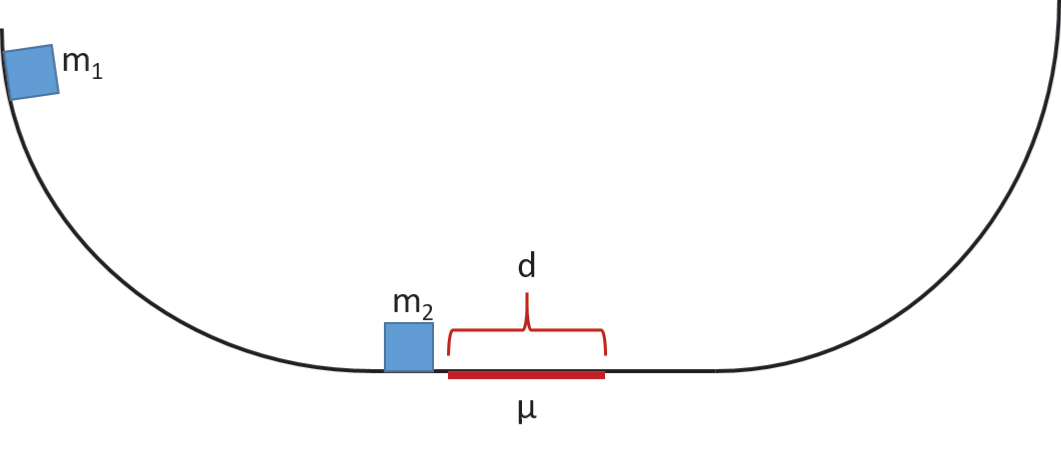
\includegraphics[width=1\textwidth]{Figures/Oppgavetegning.png}
    \figcaption{Tegning medfølgende oppgaven}
    \label{fig:oppgave}
\end{figure}

\subsection{Deloppgave (a)}
Denne oppgaven handler om bevegelsesmengde, og energibetraktning. For denne oppgaven er klossene \(m_1\) og \(m_2\) ansett som punktmasser i et friksjonløst område hvor kun tyngdekraften virker på fra utsiden av systemet.


\subsubsection{i)}
For å finne høyden til \(m_1\) i utgangspunktet kan energibetraktning gjøres. Dette krever hastigheten før kollisjonen. Dette løses med hjelp av bevaring av bevegelsesmengde. Området hvor for kollisjonen skjer er flatt og dermed er bevegelsesmengden kun langs en akse. Variabler med senket \(_f\) eller \(_e\) viser til før eller etter. Starter med å finne et uttrykk for \(v_{1f}\), farten til \(m_1\) før kollisjonen. \(m_2\) står i ro før kollisjonen, dermed er \(v_{2f} = \unitfrac[0]{m}{s}\) og dette forenkler utrykket.
\begin{equation}
\begin{split}
    p_{f} &= p_{e} \\
    m_1 v_{1f} + m_2 v_{2f} &= m_1 v_{1e} + m_2 v_{2e} \\
    m_1 v_{1f} + 0 &= m_1 v_{1e} + m_2 v_{2e} \\
    v_{1f} &= v_{1e} + \frac{m_2}{m_1} v_{2e}
\end{split}
\label{eq:v_1f}
\end{equation}

\clearpage
Siden \(m_1\) før kollisjonen er på et friksjonsfritt underlag hvor ingen ytre krefter virker inn utenom tyngdekraften er den totale mekaniske energien \(E\), bevart. Finner dermed et uttrykk for \(h_f\), høyden før klossen ble sluppet.
\begin{equation}
\begin{split}
    E_f &= E_e \\
    K_f + U_f &= K_e + U_e \\
    \frac{1}{2} m v^2_f + mgh_f &= \frac{1}{2} m v^2_e + mgh_e \\
    \frac{1}{2} v^2_f + gh_f &= \frac{1}{2} v^2_e + gh_e \\
    gh_f &= gh_e + \frac{1}{2} v^2_e  - \frac{1}{2} v^2_f \\
    gh_f &= gh_e + \frac{v^2_e  - v^2_f}{2} \\
    h_f &= h_e + \frac{v^2_e  - v^2_f}{2g}
\end{split}
\label{eq:h_generell}
\end{equation}
I start punktet er all energien i potensiell form, derfor må \(v_f = \unitfrac[0]{m}{s}\) og høyden i bunn defineres til nullpunktet slik at \(h_e = \unit[0]{m}\) med positiv retning oppover. Fyller dette inn i ligning~\ref{eq:h_generell}, Fyller også inn \(v_e = v_{1f}\), da farten før støtet er lik farten etter klossen har beveget seg ned til bunn, og deretter utrykket for \(v_{1f}\) fra ligning~\ref{eq:v_1f}.
\begin{equation}
\begin{split}
    h_f &= 0 + \frac{v^2_{1f}  - 0}{2g} \\
    h_f &= \frac{v^2_{1f}}{2g} \\
    h_f &= \frac{1}{2g} v^2_{1f} \\
    h_f &= \frac{1}{2g} \left( v_{1e} + \frac{m_2}{m_1} v_{2e} \right)^2
\end{split}
\label{eq:h}
\end{equation}
Til slutt settes verdier inn i ligning~\ref{eq:h} og høyden regnes ut.
\begin{equation*}
\begin{split}
    h_f &= \frac{1}{2 \cdot \unitfrac[9.8]{m}{s^2}} \left( \unitfrac[0,75]{m}{s} + \frac{\unit[0,30]{kg} }{\unit[0,50]{kg}} \unitfrac[3,75]{m}{s}\right)^2 \\
    h_f &\approx \unit[0,459]{m} \approx \unit[45,9]{cm}
\end{split}
\end{equation*}

Høyden \(m_1\) startet på er \underline{\underline{\(h = \unit[45,9]{cm}\)}}.

\clearpage
\subsubsection{ii)}
Hvis kollisjonen er elastisk er også den mekaniske energien \(E\) bevart i kollisjonen, ettersom det er ingen endring i høyde, faller den potensielle energien \(U\) bort og kun den kinetiske energien \(K\) er det som er bevart. \(K_{m_2f} = \unit[0]{J}\) da det er ingen kinetisk energi siden \(m_2\) står i ro før kollisjonen. Fyller også inn uttrykket for \(v_{1f}\) fra ligning~\ref{eq:v_1f}.
\begin{equation}
\begin{split}
    K_f &= K_e \\
    K_{m_1f} + K_{m_2f} &= K_{m_1e} + K_{m2e} \\
    \frac{1}{2}m_1 v^2_{1f} + 0 &= \frac{1}{2}m_1 v^2_{1e} + \frac{1}{2}m_2 v^2_{2e} \\
    m_1 v^2_{1f} &= m_1 v^2_{1e} + m_2 v^2_{2e} \\
    m_1 \left(v_{1e} + \frac{m_2}{m_1} v_{2e}\right)^2 &= m_1 v^2_{1e} + m_2 v^2_{2e} \\
    m_1 \left(v^2_{1e} + 2\frac{m_2}{m_1} v_{2e}v_{1e} + \left(\frac{m_2}{m_1} v_{2e}\right)^2\right) &= m_1 v^2_{1e} + m_2 v^2_{2e} \\
    m_1v^2_{1e} + 2m_2 v_{2e}v_{1e} + m_1\left(\frac{m_2}{m_1} v_{2e}\right)^2 &= m_1 v^2_{1e} + m_2 v^2_{2e} \\
    2m_2 v_{2e}v_{1e} + \frac{m^2_2}{m_1} v^2_{2e} &= m_2 v^2_{2e} \\
    2v_{2e}v_{1e} + \frac{m_2}{m_1} v^2_{2e} &= v^2_{2e} \\
    2v_{1e} + \frac{m_2}{m_1} v_{2e} &= v_{2e} \\
    2\frac{v_{1e}}{v_{2e}} + \frac{m_2}{m_1} &= 1 \\
\end{split}
\label{eq:K_bevart}
\end{equation}

Fyller inn verdier i ligning~\ref{eq:K_bevart} og finner ut om energien er bevart.
\begin{equation*}
\begin{split}
    2\frac{\unitfrac[0,75]{m}{s}}{\unitfrac[3,75]{m}{s}} + \frac{\unit[0,30]{kg}}{\unit[0,50]{kg}} &= 1 \\
    1 &= 1
\end{split}
\end{equation*}

Det vises tydelig at den mekaniske energien er bevart, \underline{\underline{kollisjonen er elastisk.}}

\clearpage
\subsection{Deloppgave (b)}
Denne oppgaven handler om krefter og arbeid. For denne oppgaven har \(m_1\) og \(m_2\) ingen bredde, da en bredde på klossene ville påvirket hvordan friksjonsfeltet påvirker klossene. Friksjonsfeltet \(d\) har en bredde på \(\unit[90]{cm}\) med en friksjonskoeffisient \(\mu = 0.50\).

\subsubsection{i)}
Starter med å beregne kreftene på hver kloss, kreftene som virker inn er \(G\), \(N\) og \(R\). Ser på disse som skalare størrelser da retningen på alle kreftene er kjent.
\begin{subequations}
\begin{align}
    G &= mg \\
    N &= G \\
    R &= \mu N
\end{align}
\label{eq:F}
\end{subequations}

Starter med å sette inn \(m\), \(g\) og \(\mu\) for begge klossene i ligningsystemet~\ref{eq:F} for å finne størrelsen på kreftene.
\begin{equation*}
\begin{split}
    G_{m_1} &= \unit[0,50]{kg} \cdot \unitfrac[9,8]{m}{s^2} \\
    G_{m_1} &= \unit[4,9]{N} \\
    N_{m_1} & = \unit[4,9]{N} \\
    R_{m_1} & = 0.50 \cdot \unit[4,9]{N} \\
    R_{m_1} & = \unit[2,45]{N}
\end{split}
\end{equation*}
\begin{equation*}
\begin{split}
    G_{m_2} &= \unit[0,30]{kg} \cdot \unitfrac[9,8]{m}{s^2} \\
    G_{m_2} &= \unit[2,94]{N} \\
    N_{m_2} &= \unit[2,94]{N} \\
    R_{m_2} & = 0.50 \cdot \unit[2,94]{N} \\
    R_{m_2} & = \unit[1,47]{N}
\end{split}
\end{equation*}

Fritt legeme diagram med krefter og retninger i figur~\ref{fig:fritt_legeme} på neste side.

\clearpage
\begin{figure}[h]
    \centering
    
    \begin{subfigure}{1\textwidth}
    \centering
        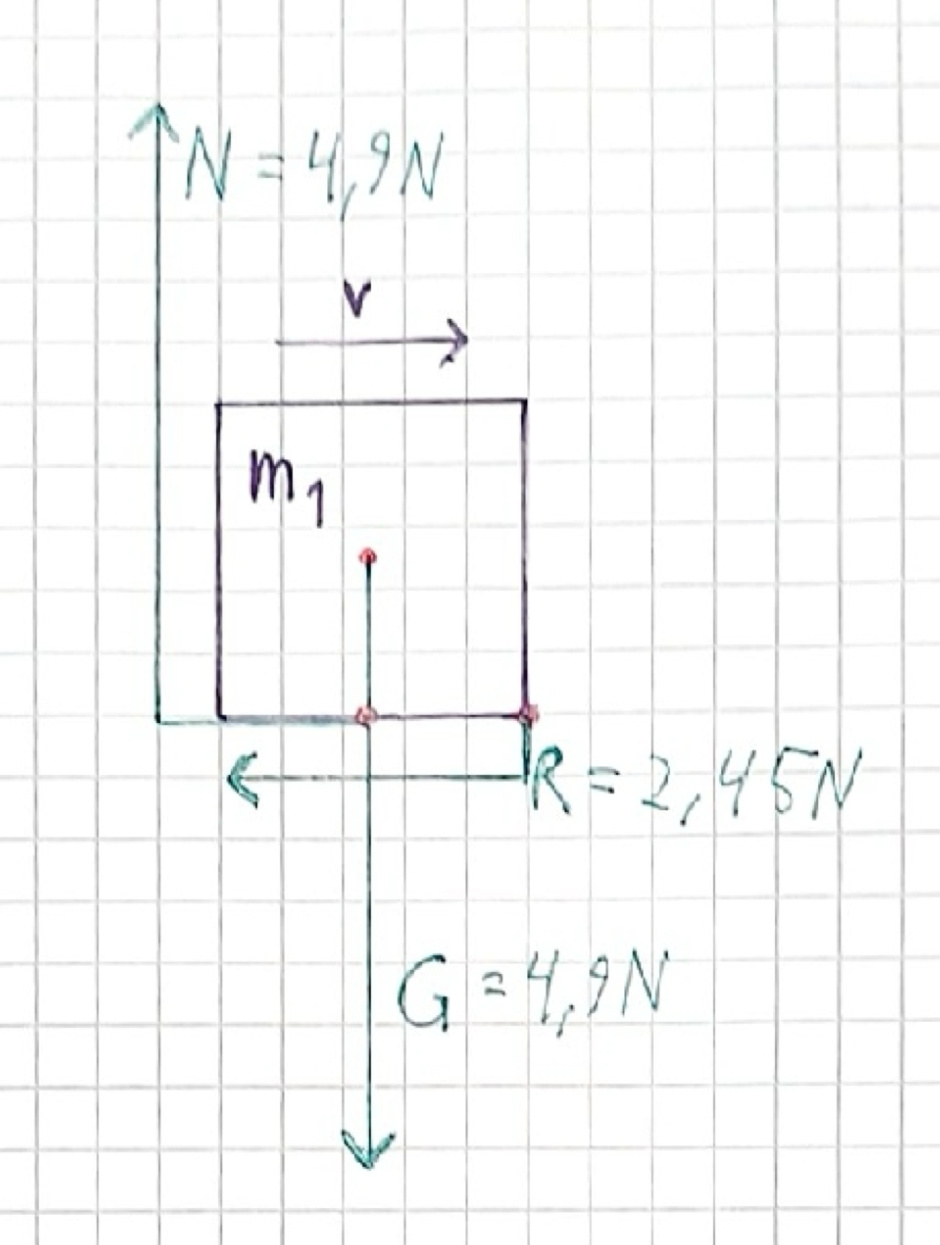
\includegraphics[width=0.6\textwidth]{Figures/m1.jpg}
        \caption{Diagram for \(m_1\)}
        \label{fig:m1}
    \end{subfigure}
    
    \begin{subfigure}{1\textwidth}
    \centering
        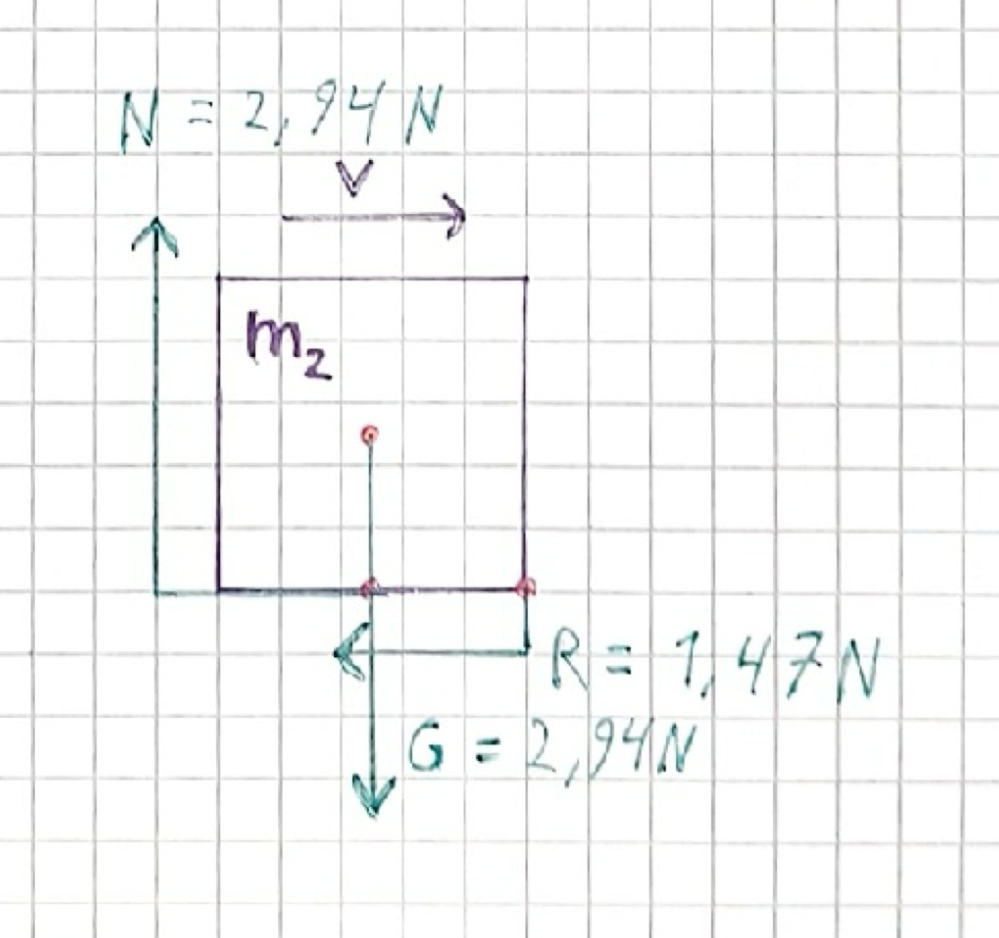
\includegraphics[width=0.6\textwidth]{Figures/m2.jpg}
        \caption{Diagram for \(m_2\)}
        \label{fig:m2}
    \end{subfigure}

    \figcaption{Fritt legeme diagram for klossene}
    \label{fig:fritt_legeme}
\end{figure}

\clearpage
\subsubsection{ii)}
Tyngdekraften \(G\) og normalkraften \(N\) er ortogonalt på bevegelsen og dermed utgjør de ingen arbeid på klossene. \(R\) er i motsatt retning til bevegelsen og dermed utgjør det et negativt arbeid på klossene. Starter med å beregne arbeidet.
\begin{equation}
\begin{split}
    W &= Fs \\
    W_R &= Rs
\end{split}
\label{eq:Wr}
\end{equation}
Fyller inn \(R\) for hver kloss i ligning~\ref{eq:Wr}, og strekningen som friksjonskraften virker på er bare på friksjonsfeltet \(d = \unit[0,90]{m}\).
\begin{equation*}
\begin{split}
    W_{R_{m_1}} &= - R_{m_1} d \\
    W_{R_{m_1}} &= - \unit[2,45]{N} \cdot \unit[0,90]{m} \\
    W_{R_{m_1}} &\approx - \unit[2,21]{J}
\end{split}
\end{equation*}
\begin{equation*}
\begin{split}
    W_{R_{m_2}} &= - R_{m_2} d \\
    W_{R_{m_2}} &= - \unit[1,47]{N} \cdot \unit[0,90]{m} \\
    W_{R_{m_2}} &\approx - \unit[1,32]{J}
\end{split}
\end{equation*}

Dette må sjekkes om er fornuftig, fordi hvis beregningen viser \(K + W_R < 0\) så stopper klossen og da er i realiteten \(W_R = - K\) istedet. Beregner \(K\) fra hastigheten etter kollisjonen.
\begin{equation*}
\begin{split}
    K_{m_1} &= \frac{1}{2} m_1 v^2_{1e} \\
    K_{m_1} &= \frac{1}{2} \unit[0,50]{kg} \cdot (\unitfrac[0,75]{m}{s})^2 \\
    K_{m_1} &\approx \unit[0,141]{J}
\end{split}
\end{equation*}
\begin{equation*}
\begin{split}
    K_{m_2} &= \frac{1}{2} m_2 v^2_{2e} \\
    K_{m_2} &= \frac{1}{2} \unit[0,30]{kg} \cdot (\unitfrac[3,75]{m}{s})^2 \\
    K_{m_2} &\approx \unit[2,11]{J}
\end{split}
\end{equation*}
For \(m_1\) observeres det at \(K_{m_1} + W_{R_{m_1}} < 0\) og dermed er \(W_{R_{m_1}} = - K_{m_1}\) mens for \(m_2\) så er \(K_{m_2} + W_{R_{m_2}} > 0\), dermed er beregning riktig. \par
Arbeidet friksjonsfeltet utgjør på \(m1\) er \underline{\underline{\(W_{R_{m_1}} \approx - \unit[0,141]{J}\)}} og klossen stopper, for \(m_2\) er arbeidet \underline{\underline{\(W_{R_{m_2}} \approx - \unit[1,32]{J}\)}}.

\clearpage
\subsection{Deloppgave (c)}
Denne oppgaven handler om begge de forrige oppgavene, energibetraktning og arbeid.

\subsubsection{i)}
For å finne ut hvilken kloss som oppnår den største høyden må høyden \(m_2\) oppnår, sammenlignes med utgangspunkt høyden til \(m_1\). Etter \(m_2\) har nådd sitt høyeste punkt ved første runde opp vil det på grunn av tap i friksjonsfeltet ikke være mulig å oppnå en høyere høyde. Starter med å lage et uttrykk for høyden til \(m_2\) med hjelp av ligning~\ref{eq:h_generell} hvor vi "bytter" før og etter på alle ledd da dette er er symetrisk forhold. setter også inn at hastigheten i topp er \(\unitfrac[0]{m}{s}\) og høyden i bunn er \(\unit[0]{m}\).
\begin{equation}
\begin{split}
    h_{m_2} = 0 + \frac{v^2_{m_2} - 0}{2 g} \\
    h_{m_2} = \frac{v^2_{m_2}}{2 g}
\end{split}
\label{eq:h_m2}
\end{equation}

Finner et utrykk for \(v^2_{m_2}\), den kvadrerte farten til \(m_2\) etter passering av friksjonsfeltet. Deretter fyller jeg det inn i ligning~\ref{eq:h_m2}. Beregner kinetisk energi etter friksjonsfeltet med \(K_{ny} = K_{m_2} + W_{R_{m_2}}\)
\begin{equation}
\begin{split}
    \frac{1}{2} m_2 v^2_{m_2} &= K_{ny} \\
    \frac{1}{2} m_2 v^2_{m_2} &= K_{m_2} + W_{R_{m_2}}\\
    v^2_{m_2} &= \frac{2}{m_2}(K_{m_2} + W_{R_{m_2}}) \\
    h_{m_2} &= \frac{\frac{2}{m_2}(K_{m_2} + W_{R_{m_2}})}{2 g} \\
    h_{m_2} &= \frac{K_{m_2} + W_{R_{m_2}}}{m_2 g}
\end{split}
\label{eq:h_m2ny}
\end{equation}

Fyller inn kjente verdier i ligning~\ref{eq:h_m2ny} og finner høyden til \(m_2\).
\begin{equation*}
\begin{split}
    h_{m_2} &= \frac{\unit[2,11]{J} - \unit[1,32]{J}}{\unit[0,30]{kg} \unitfrac[9,8]{m}{s^2}} \\
    h_{m_2} &\approx \unit[0,269]{m} \approx \unit[26,9]{cm}
\end{split}
\end{equation*}

Ved sammenligning med høyden til \(m_1\) funnet i oppgave (a) i) \(h_{m_1} = \unit[45,9]{cm}\), så er dette større en høyden til \(m_2\), \(h_{m_2} = \unit[26,9]{cm}\). \par
Klossen med størst høyde i bevegelsen er \underline{\underline{\(m_1\) med høyden \(h = \unit[45,9]{cm}\)}}.

\clearpage
\subsubsection{ii)}
For å sjekke om klossene kommer til å kollidere på nytt, må \(m_2\) bevege seg inn i friksjonsfeltet \(d\) såpass langt at den treffer \(m_1\) som stoppet opp inni feltet. Starter med å finne ut om \(m_2\) passerer feltet eller stopper inni med hjelp av den kinetiske energien etter første passering \(K_{m_2e}\), hvis den er større en \(W_{r_{m_2}}\) vil klossene kollidere, hvis den er mindre må distanse skjekkes.
\begin{equation*}
\begin{split}
    K_{m_2e} &= K_{m_2} + W_{R_{m_2}} \\
    K_{m_2e} &= \unit[2,11]{J} - \unit[1,32]{J} \\
    K_{m_2e} &= \unit[0,79]{J}\\
\end{split}
\end{equation*}
Det er tydelig at \(\unit[0,79]{J} < \unit[1,32]{J}\) Dermed sjekkes distansen. \(m_1\) og \(m_2\) beveger seg inn i funksjonsområdet.
\begin{equation}
\begin{split}
    W &= F s \\
    s &= \frac{W}{F} \\
    s &= \frac{W_R}{R}
\end{split}
\label{eq:s}
\end{equation}
For \(m_1\) fylles inn \(W_{R_{m_1}}\) og \(R_{m_1}\) i ligning~\ref{eq:s}, for \(m_2\) fylles \(-K_{m_2e}\) for \(W_R\) da det er likt arbeidet som friksjonsfeltet gjør på \(m_2\). Positiv retning er mot høyre med nullpunkt ved venstre ende av feltet, for \(m_1\) er dette rett fram, men for \(m_2\) må \(s\) erstattes med \(\unit[0,90]{m} - s\) fordi klossen beveger seg fra høyre side, siden kraften og arbeidet vil ha samme fortegn er det likegyldig hvordan de defineres.
\begin{equation*}
\begin{split}
    s_{m_1} &= \frac{W_{R_{m_1}}}{R_{m_1}} \\
    s_{m_1} &= \frac{\unit[-0,141]{J}}{\unit[-2,45]{N}} \\
    s_{m_1} &\approx \unit[0,0576]{m} \approx \unit[5,76]{cm} \\
    \unit[0,90]{m} - s_{m_2} &= \frac{-K_{m_2e}}{R_{m_2}} \\
    - s_{m_2} &= \frac{\unit[-0,79]{J}}{\unit[-1,47]{N}} - \unit[0,90]{m} \\
    s_{m_2} &= \unit[0,90]{m} - \frac{\unit[-0,79]{J}}{\unit[-1,47]{N}} \\
    s_{m_2} &\approx \unit[0,363]{m} \approx \unit[36,3]{cm}
\end{split}
\end{equation*}
distansen mellom klossene \(d_m\) blir da
\begin{equation*}
\begin{split}
    d_m &= s_{m_2} - s_{m_1} \\
    d_m &= \unit[36,3]{cm} - \unit[5,76]{cm} \\
    d_m &\approx \unit[30,5]{cm}
\end{split}
\end{equation*}
Distansen mellom klossene \(d_m > 0\), så \underline{\underline{klossene vil ikke kollidere}} før de stopper.

\end{document}
